%!TEX root = main.tex
%%%%%%%%%%%%%%%%%%%%%%%%%%%%%%%%%%%%%%%%%%%%%%%%%%%%%%%%%%%%%%%%%%%%%%%%%%%%%%%%

\subsection{Heuristic Approach}

The heuristic approach uses isotonic regression to deduce a video-dependent relationship between the data shown to the user and the resulting average quality level based on previously recorded playback sessions.
This gives an estimate of how much non-redundant data is necessary to reach a certain quality level.
Furthermore, it allows us to estimate the difference in term of average quality between two different amounts of data.

Figure \ref{fig:heuristic} illustrates the resulting relationship for one of the videos in the data-set.
The axis to the right gives the amount of Byte shown to the user.
The axis to the left gives the resulting average playback quality.
Each (brown) dot represents one playback session.
The connected (black) dots are the isotonic regression result.

The data shown to the user is the sum of the segment sizes in Bytes 

\begin{figure}[t]
\centering
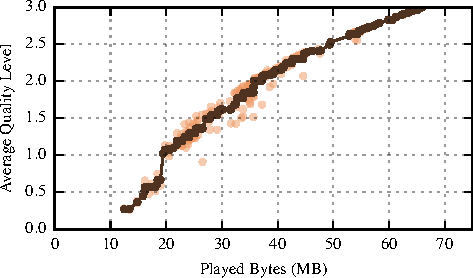
\includegraphics[width=0.9\linewidth]{figs/32_vbLLqaa9ksw.pdf}%
\caption{Isotonic regression result for video vbLLqaa9ksw.}
\label{fig:heuristic}%
\end{figure}

The advantage of the approach is that it captures the dynamics of the system.
